% IEEE journal-style manuscript. Compiles with IEEEtran (Overleaf, TeX Live full); without IEEEtran.cls a plain
% two-column fallback is used so the numbers and figures can still be checked.
\IfFileExists{IEEEtran.cls}{\documentclass[journal]{IEEEtran}\def\HAVEIEEE{1}}{\documentclass[10pt,twocolumn]{article}\usepackage[margin=0.7in,columnsep=0.25in]{geometry}}
\usepackage{amsmath,amssymb}
\usepackage{graphicx}
\usepackage{booktabs}
\usepackage[export]{adjustbox}
\usepackage[table]{xcolor}
\usepackage{microtype}
\usepackage[hyphens]{url}
\usepackage{cite}
\usepackage{hyperref}
\hypersetup{colorlinks=true,linkcolor=blue!50!black,citecolor=blue!50!black,urlcolor=blue!50!black}
\makeatletter
\@ifundefined{IEEEkeywords}{\newenvironment{IEEEkeywords}{\par\small\textbf{Index Terms---}}{\par}}{}
\@ifundefined{IEEEauthorblockN}{\newcommand{\IEEEauthorblockN}[1]{#1\\}\newcommand{\IEEEauthorblockA}[1]{#1}}{}
\makeatother
% generated by make_paper_assets.py -- do not edit
\newcommand{\agrBaseHit}{193}
\newcommand{\agrBaseK}{0.975}
\newcommand{\agrBaseN}{195}
\newcommand{\agrBaseRate}{0.990}
\newcommand{\agrBothHit}{174}
\newcommand{\agrBothK}{0.981}
\newcommand{\agrBothN}{175}
\newcommand{\agrBothRate}{0.994}
\newcommand{\appendStaleEZero}{5.00}
\newcommand{\autoDestroyedEZeroZeroFive}{0.78}
\newcommand{\autoDestroyedEZeroOne}{1.60}
\newcommand{\autoDestroyedEZeroTwo}{2.83}
\newcommand{\autoDestroyedEZeroThree}{4.60}
\newcommand{\candAdaptive}{28.1}
\newcommand{\candDefault}{8.3}
\newcommand{\candMissABase}{25}
\newcommand{\candMissABoth}{0}
\newcommand{\candMissBBase}{22}
\newcommand{\candMissBBoth}{0}
\newcommand{\carAdaptive}{0.84}
\newcommand{\carDefault}{0.04}
\newcommand{\changeTurnsA}{136}
\newcommand{\changeTurnsB}{136}
\newcommand{\cityAdaptive}{0.49}
\newcommand{\cityDefault}{0.34}
\newcommand{\destroyRedMax}{98}
\newcommand{\destroyRedMin}{94}
\newcommand{\employerAdaptive}{0.95}
\newcommand{\employerDefault}{0.18}
\newcommand{\falseAutoTwoA}{3}
\newcommand{\gateAcceptedABase}{56}
\newcommand{\gateAcceptedABoth}{68}
\newcommand{\gateAcceptedBBase}{55}
\newcommand{\gateAcceptedBBoth}{68}
\newcommand{\gateAllRatio}{2.7}
\newcommand{\gateDestroyedEZeroZeroFive}{0.05}
\newcommand{\gateDestroyedEZeroOne}{0.03}
\newcommand{\gateDestroyedEZeroTwo}{0.18}
\newcommand{\gateDestroyedEZeroThree}{0.25}
\newcommand{\gatePromptsABase}{65}
\newcommand{\gatePromptsABoth}{69}
\newcommand{\gatePromptsBBase}{68}
\newcommand{\gatePromptsBBoth}{72}
\newcommand{\gatePromptsMax}{33}
\newcommand{\gatePromptsMin}{20}
\newcommand{\gateRejectedA}{0}
\newcommand{\gateRejectedB}{0}
\newcommand{\latBaseA}{5.61}
\newcommand{\latBaseB}{6.15}
\newcommand{\latBothA}{9.39}
\newcommand{\latBothB}{5.74}
\newcommand{\lmeCtxGateB}{9}
\newcommand{\lmeCtxGateC}{0}
\newcommand{\lmeCtxGateP}{0.004}
\newcommand{\lmeGateB}{0}
\newcommand{\lmeGateC}{5}
\newcommand{\lmeGateMemPrompts}{0.9}
\newcommand{\lmeQ}{30}
\newcommand{\lmeappendBase}{0.400}
\newcommand{\lmeappendBoth}{0.333}
\newcommand{\lmeappendDiff}{$-$0.067}
\newcommand{\lmeappendP}{0.625}
\newcommand{\lmeappendStrictBase}{0.333}
\newcommand{\lmeappendStrictBoth}{0.300}
\newcommand{\lmeautoBase}{0.467}
\newcommand{\lmeautoBoth}{0.500}
\newcommand{\lmeautoDiff}{+0.033}
\newcommand{\lmeautoP}{1.000}
\newcommand{\lmeautoStrictBase}{0.333}
\newcommand{\lmeautoStrictBoth}{0.400}
\newcommand{\lmecontextBase}{0.767}
\newcommand{\lmecontextBoth}{0.733}
\newcommand{\lmecontextDiff}{$-$0.033}
\newcommand{\lmecontextP}{1.000}
\newcommand{\lmecontextStrictBase}{0.600}
\newcommand{\lmecontextStrictBoth}{0.567}
\newcommand{\lmegateBase}{0.267}
\newcommand{\lmegateBoth}{0.433}
\newcommand{\lmegateDiff}{+0.167}
\newcommand{\lmegateP}{0.063}
\newcommand{\lmegateStrictBase}{0.200}
\newcommand{\lmegateStrictBoth}{0.367}
\newcommand{\lmenoneBase}{0.000}
\newcommand{\lmenoneBoth}{0.000}
\newcommand{\lmenoneDiff}{+0.000}
\newcommand{\lmenoneP}{1.000}
\newcommand{\lmenoneStrictBase}{0.000}
\newcommand{\lmenoneStrictBoth}{0.000}
\newcommand{\mixedAdaptive}{0.866}
\newcommand{\mixedDefault}{0.286}
\newcommand{\mixedNomin}{0.607}
\newcommand{\mixedSentence}{0.690}
\newcommand{\outTokBaseA}{833}
\newcommand{\outTokBaseB}{932}
\newcommand{\outTokBothA}{796}
\newcommand{\outTokBothB}{939}
\newcommand{\personasMissBase}{10}
\newcommand{\personasStaleBase}{10}
\newcommand{\personasStaleBoth}{0}
\newcommand{\reachChanges}{2610}
\newcommand{\reachLast}{0.690}
\newcommand{\reachLastNoMin}{0.911}
\newcommand{\reachStores}{30}
\newcommand{\reachZero}{0.898}
\newcommand{\realAautofOneBase}{0.908}
\newcommand{\realAautofOneBoth}{0.956}
\newcommand{\realAautofOneDiff}{+0.048}
\newcommand{\realAautofOneHi}{0.076}
\newcommand{\realAautofOneLo}{0.019}
\newcommand{\realAautofOneP}{0.109}
\newcommand{\realAautopromptTokensBase}{13202}
\newcommand{\realAautopromptTokensBoth}{18049}
\newcommand{\realAautopromptTokensDiff}{+4847}
\newcommand{\realAautopromptTokensP}{\ensuremath{<}0.001}
\newcommand{\realAautopromptsPerOneZeroZeroTurnsBase}{0.0}
\newcommand{\realAautopromptsPerOneZeroZeroTurnsBoth}{0.0}
\newcommand{\realAautopromptsPerOneZeroZeroTurnsDiff}{+0.0}
\newcommand{\realAautopromptsPerOneZeroZeroTurnsHi}{0.00}
\newcommand{\realAautopromptsPerOneZeroZeroTurnsLo}{0.00}
\newcommand{\realAautopromptsPerOneZeroZeroTurnsP}{1.000}
\newcommand{\realAautostaleBase}{1.00}
\newcommand{\realAautostaleBoth}{0.00}
\newcommand{\realAautostaleDiff}{$-$1.00}
\newcommand{\realAautostaleHi}{-0.67}
\newcommand{\realAautostaleLo}{-1.33}
\newcommand{\realAautostaleP}{0.002}
\newcommand{\realAgatefOneBase}{0.905}
\newcommand{\realAgatefOneBoth}{0.982}
\newcommand{\realAgatefOneDiff}{+0.077}
\newcommand{\realAgatefOneHi}{0.114}
\newcommand{\realAgatefOneLo}{0.037}
\newcommand{\realAgatefOneP}{0.021}
\newcommand{\realAgatefOnefOneP}{0.625}
\newcommand{\realAgatefOnefOneVal}{0.897}
\newcommand{\realAgatefOnefTwoP}{0.146}
\newcommand{\realAgatefOnefTwoVal}{0.953}
\newcommand{\realAgatepromptTokensBase}{13376}
\newcommand{\realAgatepromptTokensBoth}{18072}
\newcommand{\realAgatepromptTokensDiff}{+4696}
\newcommand{\realAgatepromptTokensP}{\ensuremath{<}0.001}
\newcommand{\realAgatepromptsPerOneZeroZeroTurnsBase}{23.3}
\newcommand{\realAgatepromptsPerOneZeroZeroTurnsBoth}{24.9}
\newcommand{\realAgatepromptsPerOneZeroZeroTurnsDiff}{+1.6}
\newcommand{\realAgatepromptsPerOneZeroZeroTurnsHi}{3.38}
\newcommand{\realAgatepromptsPerOneZeroZeroTurnsLo}{-0.27}
\newcommand{\realAgatepromptsPerOneZeroZeroTurnsP}{0.289}
\newcommand{\realAgatestaleBase}{1.00}
\newcommand{\realAgatestaleBoth}{0.00}
\newcommand{\realAgatestaleDiff}{$-$1.00}
\newcommand{\realAgatestaleHi}{-0.67}
\newcommand{\realAgatestaleLo}{-1.33}
\newcommand{\realAgatestaleP}{0.002}
\newcommand{\realAgatestalefOneP}{1.000}
\newcommand{\realAgatestalefOneVal}{1.08}
\newcommand{\realAgatestalefTwoP}{0.021}
\newcommand{\realAgatestalefTwoVal}{0.33}
\newcommand{\realAutoLostAll}{7}
\newcommand{\realAutoLostBase}{5}
\newcommand{\realAutoRuns}{72}
\newcommand{\realBautofOneBase}{0.840}
\newcommand{\realBautofOneBoth}{0.892}
\newcommand{\realBautofOneDiff}{+0.053}
\newcommand{\realBautofOneHi}{0.076}
\newcommand{\realBautofOneLo}{0.031}
\newcommand{\realBautofOneP}{0.012}
\newcommand{\realBautopromptTokensBase}{13231}
\newcommand{\realBautopromptTokensBoth}{18090}
\newcommand{\realBautopromptTokensDiff}{+4859}
\newcommand{\realBautopromptTokensP}{\ensuremath{<}0.001}
\newcommand{\realBautopromptsPerOneZeroZeroTurnsBase}{0.0}
\newcommand{\realBautopromptsPerOneZeroZeroTurnsBoth}{0.0}
\newcommand{\realBautopromptsPerOneZeroZeroTurnsDiff}{+0.0}
\newcommand{\realBautopromptsPerOneZeroZeroTurnsHi}{0.00}
\newcommand{\realBautopromptsPerOneZeroZeroTurnsLo}{0.00}
\newcommand{\realBautopromptsPerOneZeroZeroTurnsP}{1.000}
\newcommand{\realBautostaleBase}{0.92}
\newcommand{\realBautostaleBoth}{0.00}
\newcommand{\realBautostaleDiff}{$-$0.92}
\newcommand{\realBautostaleHi}{-0.75}
\newcommand{\realBautostaleLo}{-1.00}
\newcommand{\realBautostaleP}{\ensuremath{<}0.001}
\newcommand{\realBgatefOneBase}{0.845}
\newcommand{\realBgatefOneBoth}{0.901}
\newcommand{\realBgatefOneDiff}{+0.057}
\newcommand{\realBgatefOneHi}{0.073}
\newcommand{\realBgatefOneLo}{0.038}
\newcommand{\realBgatefOneP}{0.002}
\newcommand{\realBgatepromptTokensBase}{13347}
\newcommand{\realBgatepromptTokensBoth}{18394}
\newcommand{\realBgatepromptTokensDiff}{+5047}
\newcommand{\realBgatepromptTokensP}{\ensuremath{<}0.001}
\newcommand{\realBgatepromptsPerOneZeroZeroTurnsBase}{24.5}
\newcommand{\realBgatepromptsPerOneZeroZeroTurnsBoth}{26.0}
\newcommand{\realBgatepromptsPerOneZeroZeroTurnsDiff}{+1.5}
\newcommand{\realBgatepromptsPerOneZeroZeroTurnsHi}{3.61}
\newcommand{\realBgatepromptsPerOneZeroZeroTurnsLo}{-0.95}
\newcommand{\realBgatepromptsPerOneZeroZeroTurnsP}{0.180}
\newcommand{\realBgatestaleBase}{1.08}
\newcommand{\realBgatestaleBoth}{0.00}
\newcommand{\realBgatestaleDiff}{$-$1.08}
\newcommand{\realBgatestaleHi}{-0.75}
\newcommand{\realBgatestaleLo}{-1.42}
\newcommand{\realBgatestaleP}{0.002}
\newcommand{\realDestroyed}{7}
\newcommand{\realExtractionErrors}{0}
\newcommand{\realExtractions}{3324}
\newcommand{\realGateLostAll}{0}
\newcommand{\realGateRuns}{72}
\newcommand{\realPairs}{12}
\newcommand{\realTests}{48}
\newcommand{\realWrongApplied}{0}
\newcommand{\retrAuraEmpty}{0.281}
\newcommand{\retrAuraHit}{0.700}
\newcommand{\retrBelowMin}{0.293}
\newcommand{\retrNominHit}{0.891}
\newcommand{\retrQueries}{2178}
\newcommand{\simAblFbothZero}{+0.114}
\newcommand{\simAblFfOneZero}{+0.012}
\newcommand{\simAblFfTwoZero}{+0.096}
\newcommand{\simAblStalebothOne}{0.58}
\newcommand{\simAblStalebothOneBase}{1.83}
\newcommand{\simAblStalefOneOne}{1.80}
\newcommand{\simAblStalefOneOneBase}{1.83}
\newcommand{\simAblStalefTwoOne}{0.65}
\newcommand{\simAblStalefTwoOneBase}{1.83}
\newcommand{\simFOneZero}{0.865}
\newcommand{\simFOneZeroP}{0.031}
\newcommand{\simN}{60}
\newcommand{\simTests}{210}
\newcommand{\simappendEZeroOneDestroyed}{0.00}
\newcommand{\simappendEZeroThreeDestroyed}{0.00}
\newcommand{\simappendEZeroDestroyed}{0.00}
\newcommand{\simautoEZeroOneDestroyed}{1.60}
\newcommand{\simautoEZeroThreeDestroyed}{4.60}
\newcommand{\simautoEZeroDestroyed}{0.00}
\newcommand{\simgateAllEZeroOneDestroyed}{0.05}
\newcommand{\simgateAllEZeroThreeDestroyed}{0.40}
\newcommand{\simgateAllEZeroDestroyed}{0.00}
\newcommand{\simgateEZeroOneDestroyed}{0.03}
\newcommand{\simgateEZeroThreeDestroyed}{0.25}
\newcommand{\simgateEZeroDestroyed}{0.00}
\newcommand{\singleAdaptive}{0.936}
\newcommand{\slipFThree}{0.732}
\newcommand{\slipFZero}{0.808}
\newcommand{\slipStaleThree}{2.52}
\newcommand{\slipStaleZero}{1.75}
\newcommand{\tokInc}{35}
\newcommand{\userTurnsPersona}{23}


\newcommand{\aura}{AURA}
\graphicspath{{figures/}}

\begin{document}

\title{A Review Gate Stops Wrong Memory Writes but Not Missed Updates: Candidate Selection in User-Controlled Long-Term Memory for LLM Assistants}

\author{\IEEEauthorblockN{[Author name]}
\IEEEauthorblockA{Affiliation and e-mail to be added}}

\maketitle

\begin{abstract}
Assistants that keep long-term memory about their user increasingly ask for approval before they change what they believe. We ask what such an approval gate does, and does not, protect. We study a local assistant (\aura) in which a language model proposes add, update, retire and forget operations, changes to existing memories wait for the user, and old values are kept as history. In simulation (\simN\ persona runs per cell) the gate removes \destroyRedMin--\destroyRedMax\% of the true facts that automatic application destroys when the extractor errs, at \gatePromptsMin--\gatePromptsMax\ review prompts per 100 turns. It does not reduce stale facts: the extractor can only change memories that are shown in its prompt, and with default candidate selection the memory to be changed is shown for only \reachLast\ of change requests when 350 unrelated memories are stored, and for \mixedDefault\ when the change shares a message with other sentences. A candidate selection that searches sentence by sentence without a minimum score raises the latter to \mixedAdaptive. On two real Gemini models (12 personas each) the change target was missing from the prompt in \candMissABase\ and \candMissBBase\ of 136 change turns; with the new selection it was never missing, stale facts per persona fell from about 1 to 0 under the gate (sign test $p=\realAgatestaleP$ and $\realBgatestaleP$), and F1 rose by \realAgatefOneDiff\ and \realBgatefOneDiff, at about \tokInc\% more prompt tokens and no significant increase in review prompts. A rule that lets a rejected change return after the user says something new gave no measurable benefit with real models. On 30 LongMemEval knowledge-update questions the gain with the gate (\lmegateDiff) is not significant ($p=\lmegateP$), and the memory system stays below full-context answering. The evaluation harness and all result files are provided.
\end{abstract}

\begin{IEEEkeywords}
long-term memory, conversational assistants, large language models, human-in-the-loop, memory update, evaluation.
\end{IEEEkeywords}

\section{Introduction}
Large language model (LLM) assistants that remember facts about their user across conversations must decide, after every message, whether to add a fact, change one they already hold, or drop one. Mistakes are costly in two different ways. A \emph{wrong write} replaces or removes something that was true (``moved to Pune'' overwrites the true employer), and a \emph{missed update} leaves an outdated value active after the user has said that it changed. A growing line of work treats wrong writes as a governance problem and proposes checks before a memory is stored \cite{lam2026ssgm}. A direct form of such a check is to ask the user: changes to existing memories become proposals that the user accepts or rejects, and old values are kept as history.

This paper starts from a simple observation about where such a gate sits. It acts on the operations that the extractor model \emph{returns}. An update that the extractor never produces cannot be proposed, and therefore cannot be approved. In a retrieval-based design the extractor can change only the memories that are placed in its prompt, so the choice of these candidates bounds how many updates are possible at all. We therefore ask three questions about a user-controlled memory: (Q1) How much of the damage of extractor errors does the gate remove, and at what cost in user prompts? (Q2) How often is the memory that a change refers to visible to the extractor, and how does this depend on the size of the store and on how the candidates are chosen? (Q3) Does a better candidate selection translate into fewer stale facts with real models, and what does it cost?

We study these questions in \aura, a local assistant with a SQLite memory store, local sentence embeddings and a Gemini extractor, using the assistant's real server code throughout. Our contributions are:
\begin{enumerate}
\item We separate wrong writes from missed updates and measure both under a controlled error model. The gate cuts destroyed true facts by \destroyRedMin--\destroyRedMax\% but leaves stale facts essentially unchanged (Sec.~\ref{sec:policies}).
\item We measure \emph{reachability}, the share of change requests whose target memory is in the extractor's prompt, over store sizes from 0 to 350 and for single-sentence and mixed messages, and show that the default selection becomes the bottleneck (Sec.~\ref{sec:reach}).
\item We describe two small switches, a candidate selection that searches per sentence without a minimum score (F2) and a bounded re-proposal rule (F1), and evaluate them in an ablation in simulation and with two real Gemini models, including their cost. F2 carries the effect; F1 does not show a measurable benefit with real models (Sec.~\ref{sec:ablation}--\ref{sec:real}).
\item We report an external check on LongMemEval knowledge-update questions and state clearly what it does and does not show (Sec.~\ref{sec:lme}), and we provide the harness, the personas generator and all raw results.
\end{enumerate}
We deliberately keep claims narrow. The personas are synthetic and English, the real-model samples are small, the user is simulated, and no user study was run (Sec.~\ref{sec:threats}).

\section{Related Work}
\label{sec:related}
\textbf{Memory for conversational agents and its benchmarks.} Mem0 describes an architecture that extracts, consolidates and retrieves salient facts from conversations and evaluates it on LoCoMo \cite{chhikara2025mem0}, a benchmark of very long agent--agent conversations with question answering, summarisation and multimodal tasks \cite{maharana2024locomo}. LongMemEval benchmarks chat assistants on five long-term memory abilities, among them reasoning about updated facts, and splits memory design into indexing, retrieval and reading \cite{wu2024longmemeval}. Our work uses LongMemEval's knowledge-update questions as an external check; the benchmark does not label which proposed memory changes are right, which is why our gate there uses an oracle approximation (Sec.~\ref{sec:lme}).

\textbf{Updating and governing memory.} Lam et al.\ propose a governance framework (SSGM) that separates memory updates from task execution and applies consistency checks and permission controls before anything is stored \cite{lam2026ssgm}. Patel studies the \emph{memory-update gap}, the loss of accuracy on questions about facts that changed, and addresses it by reinforcement-learning fine-tuning of a small model \cite{patel2026supersede}. Xiong et al.\ show that adding and deleting stored experiences changes agent behaviour and that errors can compound through retrieval \cite{xiong2025memory}, and Xiao et al.\ find that errors entering through memory updates persist longer than errors entering through user questions \cite{xiao2026errors}. Zhang et al.\ place a learned gate between memory store and model that decides which \emph{retrieved} memories are admitted \cite{zhang2026memgate}. Our setting differs in three ways: the gate here is a user decision on \emph{writes}, the problem we isolate is upstream of the gate (what the extractor can see), and the remedy is inference-time candidate selection rather than training. Chu surveys security threats to agents across layers and notes that current benchmarks rarely test failures that span sessions \cite{chu2026survey}.

\textbf{Scope.} The works above were read at the level of their arXiv abstract pages for this paper, not in full; their detailed claims should be checked before they are relied upon. We make no claim about priority over any of them.

\section{System: User-Controlled Memory in \aura}
\label{sec:system}
\subsection{Memory store and operations}
\aura\ keeps memories in SQLite. A memory has text, a category (preference, personal, people, work, plan, other), a status (\texttt{active}, \texttt{superseded} or \texttt{outdated}), a pointer to the memory that replaced it, a source and its conversation, and timestamps. After each user message a Gemini model (default \texttt{gemini-3.5-flash-lite}) receives the message and a list of candidate memories and returns operations: \emph{add}, \emph{update} (replace a value), \emph{retire} (the fact no longer holds), or \emph{forget}. An update keeps the old row as \texttt{superseded} with a link to its successor; retire marks the old row \texttt{outdated}. The extractor can refer only to memory identifiers that appear in its prompt.

\subsection{The review gate}
When ``ask before changing memories'' is on (the default), \emph{add} operations are applied directly and every operation that touches an existing memory becomes a stored \emph{proposal} (action, target memory, proposed text, conversation). The user accepts or rejects it; nothing changes until then. We call this policy \textbf{gate}. The comparison policies are \textbf{append} (only additions; a changed fact is stored as a second fact), \textbf{auto} (all operations applied at once), and \textbf{gate\,all} (also new facts wait for approval; emulated in the harness, not an \aura\ setting).

\subsection{Candidate selection}
\label{sec:candidates}
The prompt contains candidate memories chosen from the store. By default these are the 12 best search matches for the user's message plus the 8 most recently created memories. Search combines the cosine similarity of MiniLM sentence embeddings \cite{wang2020minilm} (\texttt{all-MiniLM-L6-v2}, run locally) and a lexical overlap score, $0.85\cdot\cos + 0.15\cdot\mathrm{lex}$, and drops matches below a minimum score of 0.25. We evaluate four modes, selected by an environment variable:
\begin{itemize}
\item \textbf{default}: as above;
\item \textbf{no minimum}: the same, without the 0.25 cut-off;
\item \textbf{sentence}: the message is split into sentences and each is searched on its own, so that an unrelated sentence does not dilute the query;
\item \textbf{adaptive} (F2): sentence search without minimum score, and a larger number of matches (up to 24) when the message contains a change cue (words such as ``moved'', ``stopped'', ``no longer'', ``forget'').
\end{itemize}
Using F2 enlarges the prompt (Sec.~\ref{sec:cost}); the minimum score exists to keep unrelated memories out (Fig.~\ref{fig:threshold}).

\subsection{Re-proposal (F1)}
A rejected proposal normally ends the matter. With F1 a rejected change may be proposed again, at most $N$ times, but only after the user has said something new about it (we use $N=2$). The aim is to recover from a rejection that was a slip without nagging the user.

\section{Evaluation Method}
\label{sec:method}
All experiments run \aura's real server code, real SQLite schema and real local embedding model on a throw-away database. What is real and what is simulated is listed in Table~\ref{tab:real-sim}.

\begin{table}[t]
\centering\small
\caption{What is real and what is simulated.}
\label{tab:real-sim}
\adjustbox{max width=\linewidth}{\begin{tabular}{lcc}
\toprule
Part & Sim.\ runs & Real runs \\
\midrule
Store, operations, proposals, search & \aura\ code & \aura\ code \\
Sentence embeddings & MiniLM & MiniLM \\
Extractor & simulated, rate $e$ & Gemini \\
Reviewing user & simulated, slip $u$ & simulated, $u=0$ \\
Conversations & scripted personas & same personas \\
\bottomrule
\end{tabular}}
\end{table}

\subsection{Personas and ground truth}
A persona has 8 of 12 fact types (city, employer, dog, sister, diet, gym time, language, car, project, coffee, hobby, birthday) and five sessions of about \userTurnsPersona\ user turns. Facts are stated, later updated (``I've just moved to Hyderabad''), retired (``I stopped going to the gym''), forgotten on request, repeated, and mixed with distractors that must not become memories (hypotheticals, questions, assistant suggestions, facts about friends). A store starts with 30 unrelated true background facts and gains 10 between sessions, imitating earlier use. The true state is known after every turn. In the ablation runs a restating turn (``Like I said, \ldots'') follows each update, which is what F1 needs to act on.

\subsection{Simulated extractor and user}
The simulated extractor returns what a correct model would return for the turn, using only the memories shown in the prompt; a change whose target is not shown becomes an add, as a real model would do. Errors are injected at rate $e$: a correct operation is dropped, a distractor becomes a false memory, or a true memory shown to the model is retired or overwritten with a false value. All policies face the same random draws. The simulated user reviews proposals at the end of a session, accepts correct ones and rejects wrong ones, and errs with probability $u$ (default 0.05).

\subsection{Metrics}
\textbf{F1} compares the persona's active memories with the true facts. \textbf{Stale} counts active memories holding a value the user gave earlier that is no longer true. \textbf{False} counts active memories the user never stated about themselves. \textbf{Destroyed} counts true memories, persona and background, that ended up superseded, outdated or deleted by a wrong change; F1 does not see the background memories, so this is the safety metric. \textbf{Prompts/100} is the number of review cards per 100 user turns. \textbf{Reachability} is the share of change requests whose target memory is among the extractor's candidates. \textbf{Prompt tokens} are summed over a persona run.

\subsection{Real-model runs and scoring}
Real runs use Gemini as the extractor for 12 personas, one seed, with the simulated user as an oracle ($u=0$), for the policies auto and gate and four variants (baseline, F1, F2, F1+F2). They were repeated for baseline and F1+F2 with a second model (\texttt{gemini-3.1-flash-lite}). Because models word memories freely, a memory is scored by value: the automatic scorer maps each active memory to a persona fact and a label (true, stale, ended, hypothetical, third party, other). The author hand-labelled every memory of the baseline and F1+F2 runs (\agrBaseN\ and \agrBothN\ memories). There were \realExtractions\ extraction calls and \realExtractionErrors\ failed.

\subsection{Statistics}
Differences between variants are paired by persona and seed. We report the mean difference with a 95\% bootstrap interval (4000 resamples, fixed seed) and an exact two-sided sign test on the non-tied pairs. No correction for multiple tests is applied; the tests run are \simTests\ (simulated ablation) and \realTests\ (real runs), so isolated $p$-values near 0.03 should not be read as findings. Reachability is reported with Wilson intervals \cite{wilson1927}, and agreement between hand and automatic labels with Cohen's $\kappa$ \cite{cohen1960}; since there is a single annotator this measures the scorer against the annotator, not human--human agreement.

\section{Results: What the Gate Protects}
\label{sec:policies}
Fig.~\ref{fig:policies} and Table~\ref{tab:policies} compare the four policies over extractor error rates $e$ (\simN\ persona runs per cell: 20 personas, 3 seeds).

\begin{figure*}[t]
\centering
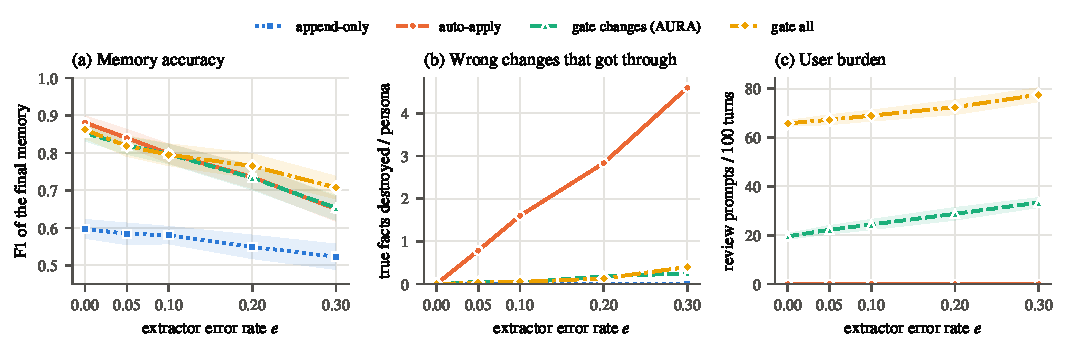
\includegraphics[width=\textwidth]{fig1_policies.pdf}
\caption{Policies under extractor errors (simulated, shaded: 95\% CI). (a) F1. (b) True facts destroyed by wrong changes. (c) Review prompts per 100 turns.}
\label{fig:policies}
\end{figure*}

\begin{table*}[t]
\centering\footnotesize
\caption{Review policies versus extractor error rate $e$ (simulated, user slip $u=0.05$, mean per persona).}
\label{tab:policies}
\adjustbox{max width=\linewidth}{\begin{tabular}{llccccc}
\toprule
$e$ & policy & F1 & stale & false & destroyed & prompts/100 \\
\midrule
0 & append-only & 0.597 $\pm$ 0.025 & 5.00 & 0.00 & 0.00 & 0.0 \\
 & auto-apply & 0.881 $\pm$ 0.018 & 1.57 & 0.00 & 0.00 & 0.0 \\
 & gate changes & 0.854 $\pm$ 0.022 & 1.80 & 0.00 & 0.00 & 19.5 \\
 & gate all & 0.861 $\pm$ 0.023 & 1.62 & 0.00 & 0.00 & 65.8 \\
\addlinespace[2pt]
0.1 & append-only & 0.581 $\pm$ 0.023 & 4.58 & 0.33 & 0.00 & 0.0 \\
 & auto-apply & 0.798 $\pm$ 0.026 & 1.68 & 0.43 & 1.60 & 0.0 \\
 & gate changes & 0.797 $\pm$ 0.026 & 1.85 & 0.33 & 0.03 & 24.4 \\
 & gate all & 0.795 $\pm$ 0.029 & 1.83 & 0.02 & 0.05 & 69.0 \\
\addlinespace[2pt]
0.3 & append-only & 0.523 $\pm$ 0.034 & 3.87 & 1.20 & 0.00 & 0.0 \\
 & auto-apply & 0.650 $\pm$ 0.032 & 1.92 & 1.33 & 4.60 & 0.0 \\
 & gate changes & 0.653 $\pm$ 0.033 & 2.18 & 1.22 & 0.25 & 33.4 \\
 & gate all & 0.707 $\pm$ 0.030 & 1.98 & 0.07 & 0.40 & 77.6 \\
\bottomrule
\end{tabular}
}
\end{table*}

\textbf{Wrong writes.} Under auto-apply the extractor's errors destroy true facts: \autoDestroyedEZeroZeroFive, \autoDestroyedEZeroOne, \autoDestroyedEZeroTwo\ and \autoDestroyedEZeroThree\ per persona at $e=0.05,0.1,0.2,0.3$. The gate reduces this to \gateDestroyedEZeroZeroFive, \gateDestroyedEZeroOne, \gateDestroyedEZeroTwo\ and \gateDestroyedEZeroThree, i.e.\ by \destroyRedMin--\destroyRedMax\%. The remainder comes from the simulated user's slips. The price is \gatePromptsMin--\gatePromptsMax\ review prompts per 100 turns; requiring approval for new facts as well removes false new facts but needs about \gateAllRatio\ times as many prompts as the gate.

\textbf{Missed updates.} The gate does not help here. At $e=0$ the append-only policy leaves \appendStaleEZero\ stale facts per persona by construction, and the gate still leaves 1.80, slightly more than auto-apply (1.57); across the error sweep the gate leaves between 1.8 and 2.2 stale facts, auto-apply between 1.6 and 1.9. F1 of the gate is below auto-apply at $e=0$ (0.854 vs.\ 0.881) and about equal at higher $e$. The gate thus buys safety at a small cost in F1, and does nothing for stale facts.

\textbf{User slips.} Table~\ref{tab:slip} varies the simulated user's slip rate at $e=0.1$. F1 falls from \slipFZero\ to \slipFThree\ and stale facts rise from \slipStaleZero\ to \slipStaleThree\ as $u$ goes from 0 to 0.3: a gate is only as good as the review.

\begin{table}[t]
\centering\small
\caption{Gate under user slips (simulated, $e=0.1$).}
\label{tab:slip}
\adjustbox{max width=\linewidth}{\begin{tabular}{ccccc}
\toprule
slip $u$ & F1 & stale & wrong changes applied & prompts/100 \\
\midrule
0 & 0.808 $\pm$ 0.026 & 1.75 & 0.02 & 24.5 \\
0.1 & 0.783 $\pm$ 0.028 & 2.00 & 0.28 & 24.4 \\
0.2 & 0.757 $\pm$ 0.027 & 2.33 & 0.42 & 24.0 \\
0.3 & 0.732 $\pm$ 0.029 & 2.52 & 0.62 & 24.1 \\
\bottomrule
\end{tabular}
}
\end{table}

\section{Results: What the Extractor Can See}
\label{sec:reach}
For each of \reachStores\ stores per size we generated update, retire and forget requests (\reachChanges\ in all) and checked whether the memory the request refers to is among the extractor's candidates. The store holds $N$ unrelated memories besides the ones the persona has stated.

\begin{figure}[t]
\centering
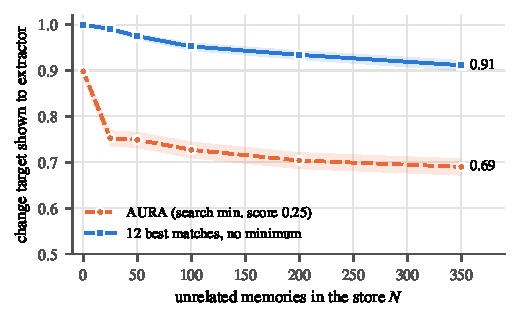
\includegraphics[width=\columnwidth]{fig3_reachability.pdf}
\caption{Share of change requests whose target memory is shown to the extractor, versus store size $N$ (shaded: Wilson 95\% CI).}
\label{fig:reach}
\end{figure}

\begin{table}[t]
\centering\small
\caption{Reachability for single-sentence changes (95\% Wilson interval).}
\label{tab:reach}
\adjustbox{max width=\linewidth}{\begin{tabular}{rcc}
\toprule
$N$ & shown (default) & shown (no minimum score) \\
\midrule
0 & 0.898 [0.886, 0.909] & 1.000 [0.999, 1.000] \\
25 & 0.752 [0.736, 0.769] & 0.990 [0.986, 0.994] \\
50 & 0.749 [0.732, 0.765] & 0.975 [0.968, 0.980] \\
100 & 0.727 [0.710, 0.744] & 0.952 [0.944, 0.960] \\
200 & 0.704 [0.686, 0.721] & 0.934 [0.924, 0.943] \\
350 & 0.690 [0.672, 0.707] & 0.911 [0.900, 0.922] \\
\bottomrule
\end{tabular}
}
\end{table}

Reachability falls from \reachZero\ with an empty store to \reachLast\ at $N=350$ (Fig.~\ref{fig:reach}, Table~\ref{tab:reach}). Even with an empty store about one change in ten is out of reach because the 0.25 minimum drops weak matches. Without the minimum the figure is \reachLastNoMin\ at $N=350$. The recent-memory slots help only at small $N$.

Table~\ref{tab:modes} compares the modes, with the mean number of candidates in parentheses. When the change shares the message with two unrelated sentences, which is common in natural conversation, default selection reaches only \mixedDefault\ of changes at $N=350$, because the embedding of the whole message is dominated by the unrelated content. Removing the minimum score gives \mixedNomin; per-sentence search alone \mixedSentence; and the adaptive mode \mixedAdaptive, at \candAdaptive\ candidates on average instead of \candDefault. Per-sentence search makes a mixed message behave like a single sentence. The minimum score is not free to remove, because it also suppresses unrelated matches (Fig.~\ref{fig:threshold}), and a larger prompt costs tokens.

\begin{table}[t]
\centering\small
\caption{Reachability by selection mode (mean number of candidates in parentheses).}
\label{tab:modes}
\adjustbox{max width=\linewidth}{\begin{tabular}{llcccc}
\toprule
$N$ & turn type & default & no min. & sentence & adaptive \\
\midrule
0 & single sentence & 0.898 (8.2) & 1.000 (11.4) & 0.898 (8.2) & 1.000 (11.4) \\
 & mixed turn & 0.747 (8.1) & 0.998 (11.4) & 0.898 (8.2) & 1.000 (11.9) \\
\addlinespace[2pt]
350 & single sentence & 0.690 (11.3) & 0.911 (19.8) & 0.690 (11.3) & 0.936 (28.2) \\
 & mixed turn & 0.286 (8.3) & 0.607 (19.8) & 0.690 (11.3) & 0.866 (28.1) \\
\bottomrule
\end{tabular}
}
\end{table}

\begin{figure}[t]
\centering
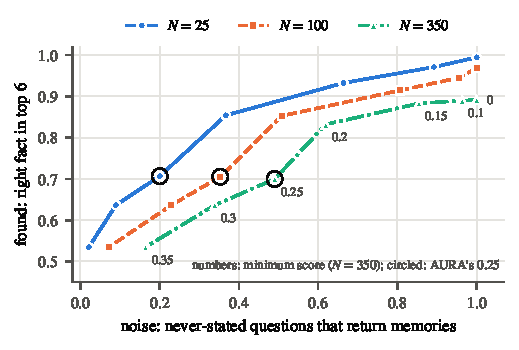
\includegraphics[width=\columnwidth]{fig4_threshold_tradeoff.pdf}
\caption{Retrieval trade-off of the minimum score: share of stored facts found in the top six versus share of never-stated questions that still return memories. Circled: \aura's 0.25.}
\label{fig:threshold}
\end{figure}

\section{Results: Ablation of the Two Switches}
\label{sec:ablation}
\subsection{Simulated}
Table~\ref{tab:simabl} and Fig.~\ref{fig:abl} give the paired ablation under the gate (error sweep, $u=0.05$, restating turns on). F2 reduces stale facts per persona at $e=0.1$ from \simAblStalefOneOneBase\ to \simAblStalefTwoOne\ and F1+F2 to \simAblStalebothOne; the F2 effects are significant ($p<0.001$) in every cell shown. F1 alone moves F1 by \simAblFfOneZero\ at $e=0$ ($p=\simFOneZeroP$), and is not significant at $e=0.1$ and $0.2$. With 210 tests that single $p$-value would not survive a correction. F2 raises the review load by about 5 prompts per 100 turns at $e=0.1$ because more changes are discovered and proposed.

\begin{table*}[t]
\centering\footnotesize
\caption{Ablation under the gate (simulated). In parentheses: difference to the baseline and sign-test $p$ (60 pairs).}
\label{tab:simabl}
\adjustbox{max width=\linewidth}{\begin{tabular}{llccc}
\toprule
$e$ & variant & F1 (diff., $p$) & stale (diff., $p$) & prompts/100 \\
\midrule
0 & baseline & 0.854 & 1.80 & 17.6 \\
 & +F1 & 0.865 (+0.012, 0.031) & 1.70 ($-$0.10, 0.031) & 18.3 \\
 & +F2 & 0.950 (+0.096, \ensuremath{<}0.001) & 0.40 ($-$1.40, \ensuremath{<}0.001) & 24.3 \\
 & F1+F2 & 0.967 (+0.114, \ensuremath{<}0.001) & 0.27 ($-$1.53, \ensuremath{<}0.001) & 25.0 \\
\addlinespace[2pt]
0.1 & baseline & 0.817 & 1.83 & 23.7 \\
 & +F1 & 0.821 (+0.005, 0.500) & 1.80 ($-$0.03, 0.500) & 23.9 \\
 & +F2 & 0.890 (+0.074, \ensuremath{<}0.001) & 0.65 ($-$1.18, \ensuremath{<}0.001) & 29.1 \\
 & F1+F2 & 0.901 (+0.084, \ensuremath{<}0.001) & 0.58 ($-$1.25, \ensuremath{<}0.001) & 29.4 \\
\addlinespace[2pt]
0.2 & baseline & 0.737 & 1.98 & 28.6 \\
 & +F1 & 0.747 (+0.010, 0.250) & 1.92 ($-$0.07, 0.250) & 28.8 \\
 & +F2 & 0.776 (+0.039, \ensuremath{<}0.001) & 1.22 ($-$0.77, \ensuremath{<}0.001) & 32.2 \\
 & F1+F2 & 0.784 (+0.047, \ensuremath{<}0.001) & 1.17 ($-$0.82, \ensuremath{<}0.001) & 32.7 \\
\bottomrule
\end{tabular}
}
\end{table*}

\begin{figure*}[t]
\centering
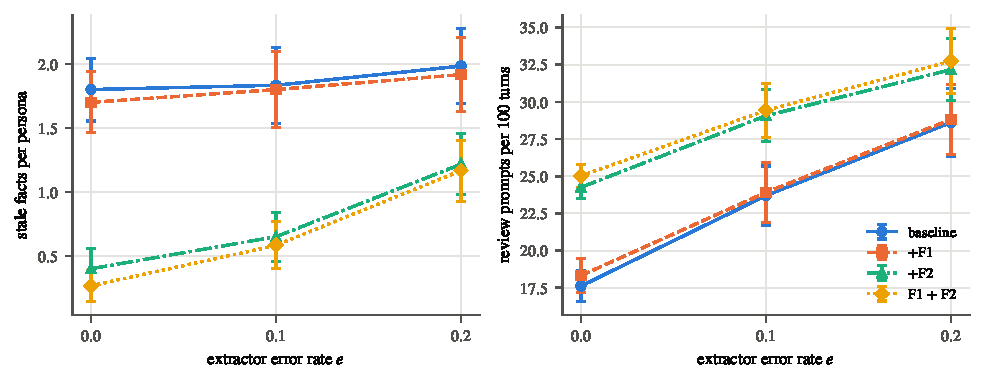
\includegraphics[width=\textwidth]{fig5_ablation.pdf}
\caption{Gate policy, error sweep: stale facts and review prompts for baseline, F1, F2, F1+F2 (simulated).}
\label{fig:abl}
\end{figure*}

\section{Results: Real Gemini Extractors}
\label{sec:real}
Table~\ref{tab:real1} and Fig.~\ref{fig:real} give the same ablation with a real extractor (12 personas, one seed, oracle user). Table~\ref{tab:real2} repeats baseline and F1+F2 with a second model.

\begin{table*}[t]
\centering\footnotesize
\caption{Real extractor \texttt{gemini-3.5-flash-lite}: 12 paired personas per cell. In parentheses: difference to the baseline and exact sign-test $p$.}
\label{tab:real1}
\adjustbox{max width=\linewidth}{\begin{tabular}{llccccc}
\toprule
policy & variant & F1 & stale & false & prompts/100 & prompt tokens ($\times10^3$) \\
\midrule
auto & baseline & 0.908 & 1.00 & 0.00 & 0.0 & 13.2 \\
 & +F1 & 0.902 ($-$0.007, 1.000) & 1.00 (+0.00, 1.000) & 0.08 (+0.08, 1.000) & 0.0 & 13.2 \\
 & +F2 & 0.943 (+0.035, 0.453) & 0.00 ($-$1.00, 0.002) & 0.25 (+0.25, 0.250) & 0.0 & 18.0 \\
 & F1+F2 & 0.956 (+0.048, 0.109) & 0.00 ($-$1.00, 0.002) & 0.00 (+0.00, 1.000) & 0.0 & 18.0 \\
\addlinespace[2pt]
gate & baseline & 0.905 & 1.00 & 0.00 & 23.3 & 13.4 \\
 & +F1 & 0.897 ($-$0.008, 0.625) & 1.08 (+0.08, 1.000) & 0.00 (+0.00, 1.000) & 21.9 & 13.3 \\
 & +F2 & 0.953 (+0.048, 0.146) & 0.33 ($-$0.67, 0.021) & 0.08 (+0.08, 1.000) & 24.2 & 18.2 \\
 & F1+F2 & 0.982 (+0.077, 0.021) & 0.00 ($-$1.00, 0.002) & 0.00 (+0.00, 1.000) & 24.9 & 18.1 \\
\bottomrule
\end{tabular}
}
\end{table*}

\begin{table*}[t]
\centering\footnotesize
\caption{Second extractor \texttt{gemini-3.1-flash-lite}: baseline versus F1+F2, 12 paired personas.}
\label{tab:real2}
\adjustbox{max width=\linewidth}{\begin{tabular}{llccccc}
\toprule
policy & variant & F1 & stale & false & prompts/100 & prompt tokens ($\times10^3$) \\
\midrule
auto & baseline & 0.840 & 0.92 & 0.00 & 0.0 & 13.2 \\
 & F1+F2 & 0.892 (+0.053, 0.012) & 0.00 ($-$0.92, \ensuremath{<}0.001) & 0.00 (+0.00, 1.000) & 0.0 & 18.1 \\
\addlinespace[2pt]
gate & baseline & 0.845 & 1.08 & 0.00 & 24.5 & 13.3 \\
 & F1+F2 & 0.901 (+0.057, 0.002) & 0.00 ($-$1.08, 0.002) & 0.00 (+0.00, 1.000) & 26.0 & 18.4 \\
\bottomrule
\end{tabular}
}
\end{table*}

\begin{figure*}[t]
\centering
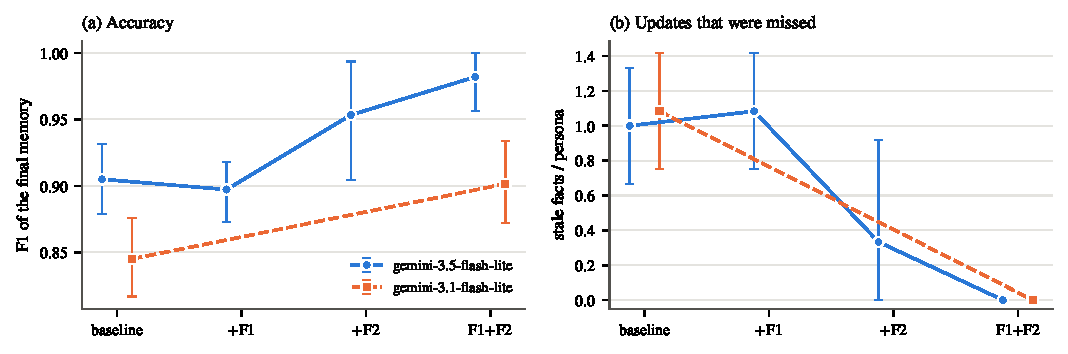
\includegraphics[width=\textwidth]{fig6_real.pdf}
\caption{Gate policy with real Gemini extractors: (a) F1, (b) stale facts per persona; mean and 95\% bootstrap interval over 12 personas.}
\label{fig:real}
\end{figure*}

\textbf{Reachability on real conversations.} With the baseline selection, the target memory was missing from the prompt on \candMissABase\ of \changeTurnsA\ change turns (first model; both policies together) and \candMissBBase\ of \changeTurnsB\ (second model). With F1+F2 it was missing on \candMissABoth\ and \candMissBBoth. This is the mechanism of Sec.~\ref{sec:reach} observed with real conversations.

\textbf{Stale facts and F1.} Under the gate, stale facts per persona fell from \realAgatestaleBase\ to \realAgatestaleBoth\ (first model; $p=\realAgatestaleP$) and from \realBgatestaleBase\ to \realBgatestaleBoth\ (second; $p=\realBgatestaleP$), and F1 rose from \realAgatefOneBase\ to \realAgatefOneBoth\ (\realAgatefOneDiff, $p=\realAgatefOneP$) and from \realBgatefOneBase\ to \realBgatefOneBoth\ (\realBgatefOneDiff, $p=\realBgatefOneP$). F2 alone reached \realAgatestalefTwoVal\ stale facts ($p=\realAgatestalefTwoP$) and F1 of \realAgatefOnefTwoVal\ ($p=\realAgatefOnefTwoP$, not significant); the benefit of adding F1 to F2 was not tested separately and is within what 12 personas can resolve. F1 alone changed nothing measurable (stale \realAgatestalefOneVal, $p=\realAgatestalefOneP$): on real models F1 is not supported. Under auto-apply the picture is the same (stale \realAautostaleBase\ to \realAautostaleBoth, $p=\realAautostaleP$).

\textbf{Safety on real models.} No injected errors exist in real runs, so we count what the models did. Across all auto-apply persona runs (\realAutoRuns), \realAutoLostAll\ true background facts were destroyed by the model's own operations (\realAutoLostBase\ of them in the two baseline runs); across the \realGateRuns\ gate runs the count was \realGateLostAll. With the oracle user, no correct change was rejected, no wrong change was accepted and \realWrongApplied\ wrong changes were applied. Because the user is perfect and the counts are small, this is a consistency check on the simulation, not a measurement of real users.

\textbf{Cost.} Prompt tokens per persona rose from about 13.4k to 18.1k (+\tokInc\%, $p<0.001$), and the number of prompts per 100 turns from \realAgatepromptsPerOneZeroZeroTurnsBase\ to \realAgatepromptsPerOneZeroZeroTurnsBoth\ (first model, $p=\realAgatepromptsPerOneZeroZeroTurnsP$) and from \realBgatepromptsPerOneZeroZeroTurnsBase\ to \realBgatepromptsPerOneZeroZeroTurnsBoth\ (second, $p=\realBgatepromptsPerOneZeroZeroTurnsP$), not significant. Of the change prompts, \gateAcceptedABoth\ of \gatePromptsABoth\ (first model) and \gateAcceptedBBoth\ of \gatePromptsBBoth\ (second) in the F1+F2 runs were correct changes that the user accepted, against \gateAcceptedABase\ of \gatePromptsABase\ and \gateAcceptedBBase\ of \gatePromptsBBase\ for the baselines; this is consistent with the added prompts being updates that the baseline missed.\label{sec:cost}

\textbf{Other effects.} Under auto-apply the F2-only variant stored \falseAutoTwoA\ false facts across 12 personas where the baseline stored none, and F1+F2 stored none again; with these counts we cannot say whether this is an effect of F2 or noise.

\subsection{Scorer validity}
Table~\ref{tab:agree} shows the agreement of the automatic labels with the author's hand labels. Three of \agrBaseN\,+\,\agrBothN\ memories differ; in all three the automatic scorer labelled a correct statement of unemployment or finished project as ``ended'' or ``other'' while the annotator judged it true, so the automatic F1 is, if anything, slightly conservative on these three. These labels were kept as annotated. Since the scorer and the labels share one author and the same persona rules, the agreement shows consistency, not independence.

\begin{table}[t]
\centering\small
\caption{Agreement between automatic and hand labels (single annotator).}
\label{tab:agree}
\adjustbox{max width=\linewidth}{\begin{tabular}{lcccc}
\toprule
run & labelled memories & agreement & rate & Cohen's $\kappa$ \\
\midrule
baseline & 195 & 193 & 0.990 & 0.975 \\
F1+F2 & 175 & 174 & 0.994 & 0.981 \\
\bottomrule
\end{tabular}
}
\end{table}

\section{External Check: LongMemEval}
\label{sec:lme}
LongMemEval's knowledge-update questions ask for the latest value of a fact that changed during the history \cite{wu2024longmemeval}. We took \lmeQ\ such questions of the ``S'' setting and played each with all evidence sessions plus three random distractor sessions (the same for every system) through \aura's extractor, store and search; answers come from the ten memories that \aura's search returns, and are graded by a Gemini judge written after the benchmark's rule (the official prompt is not reproduced) and by string match. All runs use \texttt{gemini-3.1-flash-lite}. There is no label for which memory changes are right, so the gate's reviewer is an oracle approximation: it accepts proposals made while reading an evidence session and rejects the rest. This gate figure is therefore an upper-bracket, not a measurement of real users. Baselines are answering with no memory and with the raw sessions as context.

\begin{table}[t]
\centering\small
\caption{LongMemEval knowledge-update questions (judge-graded accuracy, $n=\lmeQ$). $b/c$: questions correct only in the baseline / only in the F1+F2 run.}
\label{tab:lme}
\adjustbox{max width=\linewidth}{\begin{tabular}{lccccc}
\toprule
system & baseline & F1+F2 & difference & $b/c$ & $p$ \\
\midrule
no memory & 0.000 & 0.000 & +0.000 & 0/0 & 1.000 \\
full context & 0.767 & 0.733 & $-$0.033 & 1/0 & 1.000 \\
append-only & 0.400 & 0.333 & $-$0.067 & 3/1 & 0.625 \\
auto-apply & 0.467 & 0.500 & +0.033 & 1/2 & 1.000 \\
gate (oracle reviewer) & 0.267 & 0.433 & +0.167 & 0/5 & 0.063 \\
\bottomrule
\end{tabular}
}
\end{table}

\begin{figure}[t]
\centering
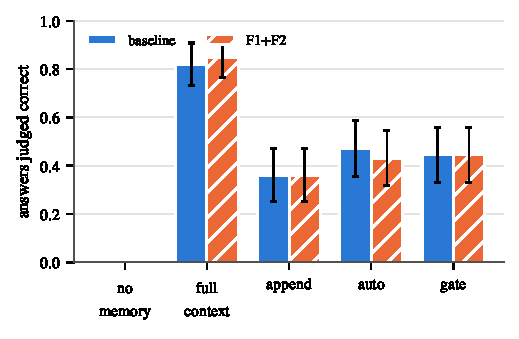
\includegraphics[width=\columnwidth]{fig7_lme.pdf}
\caption{LongMemEval accuracy by system for baseline and F1+F2 selection (95\% normal-approximation bars).}
\label{fig:lme}
\end{figure}

Table~\ref{tab:lme} and Fig.~\ref{fig:lme} show that the gate system improves from \lmegateBase\ to \lmegateBoth\ (\lmeGateB\ questions worse, \lmeGateC\ better, $p=\lmegateP$), which is in the expected direction but not significant at this sample size; the systems without memory or with full context, which cannot be affected, differ by \lmecontextDiff\ between the two runs, which indicates run-to-run noise of that size. Auto-apply and append are not distinguishable between the runs. Full-context answering (\lmecontextBoth\ in the second run) remains clearly above the gate system (\lmegateBoth; \lmeCtxGateB\ vs.\ \lmeCtxGateC\ discordant questions, $p=\lmeCtxGateP$): a memory system trades accuracy for the properties it provides, such as small prompts, forgetting and user control. A run on all 78 knowledge-update questions would be needed for a firm statement.

\section{Discussion}
\label{sec:discussion}
\textbf{Where the guarantee ends.} The gate provides a guarantee about what is \emph{written}: nothing changes without approval. It provides none about what is \emph{proposed}. In our experiments the second quantity depends on a component that looks like plumbing, the choice of candidate memories, and with default settings it is the main reason that stale facts remain. Evaluating a user-controlled memory by its write accuracy or by the number of approvals alone would miss this.

\textbf{Design implications.} (i) Report reachability alongside accuracy for any extractor-based memory. (ii) Search per sentence rather than per message when messages are mixed. (iii) Treat the minimum score as a trade-off: the unfiltered selection raises reachability (\reachLastNoMin\ at $N=350$) but admits unrelated memories, so the price of F2 is a larger prompt. (iv) Budget for more prompt tokens (about \tokInc\%) and slightly more review cards.

\textbf{On F1.} Letting a rejected change return only after new user input is cheap and conceptually neat, but we found no benefit with real models (the oracle user rejected no correct change in these runs), and only small, uncorrected-significance effects in simulation. Its value would have to be shown with real users who slip.

\section{Threats to Validity}
\label{sec:threats}
\textbf{Synthetic and English personas.} Personas, distractors and the wording of changes were written by the system's author. The change cues of F2 were designed after the reachability failures were seen on the same generator, so F2 may be tuned to it; the LongMemEval check is the only independent text and is small. \textbf{Small real samples.} 12 personas, one seed per cell and two models of the same family; exact sign tests with 12 pairs cannot resolve small effects, and several F1 results are inconclusive rather than null. \textbf{Simulated user.} The real runs use a perfect reviewer, the simulations a random slip. Real users may ignore, batch or rubber-stamp prompts; whether additional prompts are tolerated is open. No user study was done. \textbf{Single annotator and scorer.} Labels come from the author. \textbf{One embedding model.} Reachability depends on MiniLM and the 0.25 threshold. \textbf{LongMemEval.} Thirty questions, a judge that is not the official prompt, an oracle reviewer, and a single seed. \textbf{Multiple tests.} Reported as counts; only the large effects are robust to correction. \textbf{Related work.} Sources were read at abstract level.

\section{Conclusion}
A review gate on memory changes is effective against the errors it can see: in our experiments it removes almost all of the true facts that automatic application destroys. It does not address updates the extractor never proposes, and in a retrieval-based design these are governed by which memories the extractor is shown. Showing candidates by sentence, without a minimum score and with a larger set on a change cue, removed all observed misses for two real Gemini models and removed the stale facts, at roughly a third more prompt tokens and no significant increase in review prompts, while an external check on LongMemEval pointed in the same direction without reaching significance. The practical lesson for user-controlled memories is to measure and report what the extractor can reach. Evaluating with real users, in other languages and with larger real samples is the necessary next step; the evaluation code and every raw result file are provided so that others can repeat and extend it.

\section*{Data and Code Availability}
The evaluation harness (\texttt{eval/}), the persona generator, all raw per-run files and the scripts that produce every table and figure of this paper (\texttt{eval/make\_paper\_assets.py}) are in the \aura\ project repository. Numbers in the text are generated from the result folders.

\ifdefined\HAVEIEEE\bibliographystyle{IEEEtran}\else\bibliographystyle{unsrt}\fi
\bibliography{references}

\end{document}
